\section{Waveform Views}

A waveform view is a 2D graph of a signal or protocol decode within a waveform group.

\subsection{Plot Area}

The plot area shows the waveform being displayed. The background has a subtle gradient from light at top to dark at
bottom, in order to visually separate adjacent waveform view within the same group.

The horizontal grid lines line up with the voltage scale markings on the Y axis. If the plot area includes Y=0, the
grid line for zero is slightly brighter.

\begin{figure}[H]
\centering
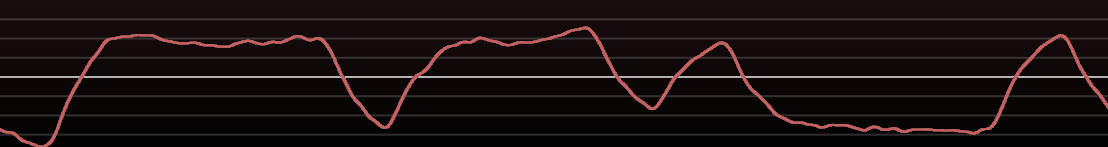
\includegraphics[width=10cm]{images/waveform-graph.png}
\caption{Waveform plot area}
\label{waveform-graph}
\end{figure}

The waveform is drawn as a semi-transparent line so that when zoomed out, the density of voltage at various points in
the graph may be seen as lighter or darker areas. This is referred to as ``intensity grading".

\begin{figure}[H]
\centering
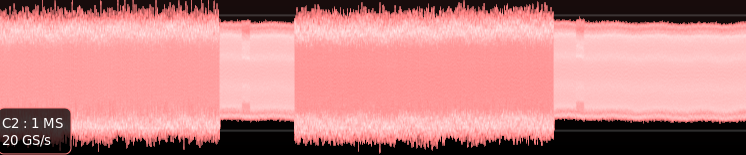
\includegraphics[width=10cm]{images/graded-waveform.png}
\caption{Intensity-graded waveform}
\label{graded-waveform2}
\end{figure}

\subsection{Y Axis Scale}

Each waveform view has its own Y axis scale, which is locked to the ADC range of the instrument.

Dragging the Y axis scale with the left mouse button currently does nothing (scopehal-apps:54) but in a future software
release will change the voltage offset of the channel.

Scrolling the Y axis scale with the mouse wheel changes the gain of the channel.

If a left-pointing arrow (as seen in Fig. \ref{y-axis}) is visible, the current channel is selected as a trigger
source. Click on the arrow and drag up or down to select the trigger level.

\begin{figure}[H]
\centering
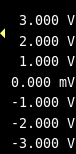
\includegraphics[height=3cm]{images/y-axis.png}
\caption{Y axis of a waveform view showing trigger arrow}
\label{y-axis}
\end{figure}

\subsection{Channel Information Box}

The channel information box is displayed in the lower left corner of each waveform view. It contains summary
information about the channel. Currently this is the display name of the channel, the sample rate, and the record
length of the acquisition. Other information, such as probe coupling, may be displayed there in the future.

Double-clicking the information box opens the channel properties dialog.

\begin{figure}[H]
\centering
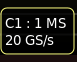
\includegraphics[width=2cm]{images/channel-infobox.png}
\caption{Channel information box}
\label{channel-infobox}
\end{figure}

\subsection{Overlays}

Waveforms may have additional information overlaid on top of them, such as protocol decodes. Each overlay has its own
information box, which may be double-clicked to open the properties dialog and configure it just like any other
channel.

Fig. \ref{overlays} shows
an example of an analog waveform with three overlays: thresholding it to NRZ digital, recovering a sampling
clock with a CDR PLL, and finally decoding the serial NRZ data stream to TMDS protocol data and control events.

\begin{figure}[H]
\centering
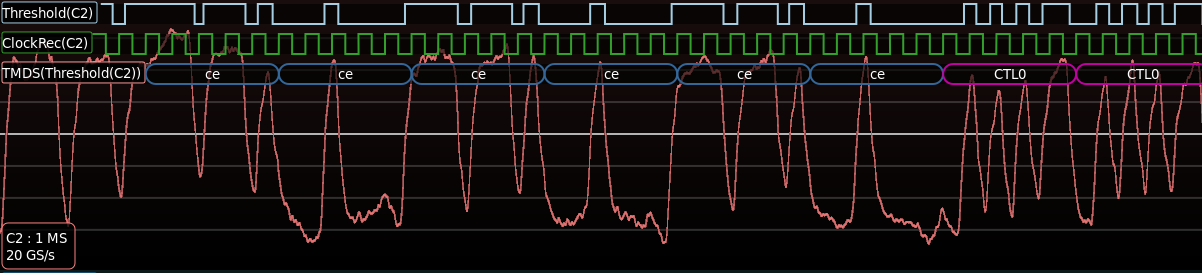
\includegraphics[width=14cm]{images/overlays.png}
\caption{Waveform showing two digital overlays and a data decode overlay}
\label{overlays}
\end{figure}

Overlays can be deleted but cannot currently be moved between waveform areas or reordered within a single waveform area
(scopehal-apps:7, scopehal-apps:6)
